\documentclass[../notes.tex]{subfiles}
\begin{document}
    \subsection{Modo matemática}

        \textbf{In-line}: se utiliza para escribir fórmulas dentro del párrafo. Se puede utilizar tanto \texttt{\$math\$} o \texttt{\textbackslash ( math \textbackslash )}.
        \textbf{Display}: se utiliza para escribir fórmulas fuera del párrafo, y por tanto, en una linea separada. Se puede utilizar tanto \texttt{\$\$math\$\$} como \texttt{\textbackslash[math\textbackslash]}.
        
        \begin{verbatim}
Como $f(x) = x^3$, entonces
    $$ \int_{a}^{b} f(x) dx = \frac{x^4}{4}.$$
De esta forma, como \(a = 0\) y \(b = 1\)
    \[ \int_{0}^{1} f(x) dx = 
    \frac{1^4}{4} - \frac{0^4}{4} = \frac{1}{4} \]
        \end{verbatim}
Como $f(x) = x^3$, entonces
    $$ \int_{a}^{b} f(x) dx = \frac{x^4}{4}.$$
De esta forma, como \(a = 0\) y \(b = 1\)
    \[ \int_{0}^{1} f(x) dx = 
    \frac{1^4}{4} - \frac{0^4}{4} = \frac{1}{4} \]
    
        Si nos interesa alinear las fórmulas, del estilo
            \begin{align}
            	x^2 - 1 = 0 &\implies x^2 = 1\\
            	&\implies x = \pm 1.
            \end{align}
        Entonces podemos utilizar el comando \texttt{align}. Este comando nos permite alinear múltiples lineas de ecuaciones a partir del simbolo de alineamiento \&.
            \begin{verbatim}
\begin{align}
    x^2 - 1 = 0 &\implies x^2 = 1\\
    &\implies x = \pm 1.
\end{align}
            \end{verbatim}

        Nota: Observe que \texttt{align} enumera cada una de las lineas del ambiente. Si no requerimos esto, entonces se puede utilizar el comando \texttt{align*}, que no enumera ecuaciones.
        
            \begin{verbatim}
\begin{align*}
    x^2 - 1 = 0 &\implies x^2 = 1\\
    &\implies x = \pm 1.
\end{align*}
            \end{verbatim}
    \begin{align*}
        x^2 - 1 = 0 &\implies x^2 = 1\\
        &\implies x = \pm 1.
    \end{align*}
    
        Nota: Por otro lado, si solo se le quiere eliminar la enumeración a una sola ecuación, entonces se puede utilizar \texttt{nonumber}
                \begin{verbatim}
\begin{align}
    \nonumber x^2 - 1 = 0 &\implies x^2 = 1\\
    &\implies x = \pm 1.
\end{align}
            \end{verbatim}
    \begin{align}
        \nonumber  x^2 - 1 = 0 &\implies x^2 = 1\\
        &\implies x = \pm 1.
    \end{align}
    
    \subsection{Notación básica}
    
        \begin{enumerate}
            \item Aritmética
                \begin{center}
                \begin{tabular}{|c|c|c|}
                \hline
                    Suma & \texttt{1 + 2 = 3} & $\quad\quad1 + 2 = 3\quad\quad$\\
                \hline
                    Resta & \texttt{8 - 1 = 7} & $8 - 1 = 7$\\
                \hline
                    Multiplicación & \texttt{3 \textbackslash cdot 4 = 12} & $3 \cdot 4 = 12$\\
                \hline
                    Multiplicación & \texttt{3 \textbackslash times 4 = 12} & $3 \times 4 = 12$\\
                \hline
                    División & \texttt{25 \textbackslash div 5 = 5} & $25 \div 5 = 5$\\
                \hline
                \end{tabular}
                \end{center}
            \item Fracciones
                \begin{center}
                \begin{tabular}{|c|c|c|}
                \hline
                    & & \\
                    Fracción & \texttt \textbackslash frac\{12\}\{48\} & $\quad\quad\dfrac{1}{4}\quad\quad$ \\
                    & & \\
                \hline
                \end{tabular}
                \end{center}
        \end{enumerate}

        Nota:
            \begin{itemize}
                \item Es buena práctica utilizar fracciones en vez de divisiones.
                \item Utilizar \texttt{frac} en modo in-line entregará una versión más compacta de esta. En caso de necesitar la versión ampliada, se puede utilizar \texttt{dfrac}. En el caso de estar en modo display, no habrá diferencia.
            \end{itemize}
        \begin{center}
           \begin{tabular}{|c|c|c|}
             \hline
                 & Modo in-line & Modo display\\
            \hline
                & & \\
                 \texttt \textbackslash frac\{12\}\{48\} & $\quad\quad\frac{1}{4}\quad\quad$ & $\quad\quad\dfrac{1}{4}\quad\quad$ \\
                        & & \\
                \texttt \textbackslash dfrac\{12\}\{48\} & $\quad\quad\dfrac{1}{4}\quad\quad$ & $\quad\quad\dfrac{1}{4}\quad\quad$ \\
                        & & \\
              \hline
          \end{tabular}
        \end{center}

    \subsection{Superlineado y sublineado}

            \textbf{Superlineado}: 

                Se utiliza \texttt{\^} para escribir en superlineado. Por ejemplo, exponentes.

                \begin{verbatim}
Se tiene entonces que 
$e^{i\pi} = -1$.
                \end{verbatim}
Se tiene entonces que $e^{i\pi} = -1$.
                \textbf{Sublineado}: 

                Se utiliza \texttt{\_} para escribir en sublineado. Por ejemplo, índices.

                \begin{verbatim}
Por tanto, existe una
subsucesión $x_{k_{j}}$.
                \end{verbatim}
Por tanto, existe una subsucesión $x_{k_{j}}$.
    
        \begin{enumerate}
            \item Limite
            
            \begin{center}
                \begin{tabular}{|c|c|}
                    \hline
                        & \\
                        \begin{tabular}{@{}c@{}} \texttt{\textbackslash lim\_\{x\textbackslash{}to\textbackslash{}infty\}  \textbackslash frac\{x\^{}2\}\{2x\^{}2+1\}}\\\texttt{ = \textbackslash frac 1 2} \end{tabular} 
                        & $\displaystyle \quad\lim_{x \to \infty} \frac{x^2}{2x^2+1} = \frac 1 2\quad$ \\
                        & \\
                    \hline
                \end{tabular}
            \end{center}

            \item Sumatoria
            
            \begin{center}
                \begin{tabular}{|c|c|}
                    \hline
                        & \\
                        
                        \texttt {\textbackslash sum\_\{x = 1\}\^{}n x = \textbackslash frac\{n(n+1)\}\{2}\} & $\displaystyle \quad\sum_{x = 1}^n x = \dfrac{n(n+1)}{2} \quad$ \\
                        & \\
                    \hline
                \end{tabular}
            \end{center}

            \item Integral
            
            \begin{center}
                \begin{tabular}{|c|c|}
                    \hline
                        & \\
                        \texttt { \textbackslash int\_\{0\}\^{}1 e\^{}x = e\^{}1 - 1} & $\displaystyle \quad\int_{0}^1 e^x = e^1 - 1\quad$ \\
                        & \\
                    \hline
                \end{tabular}
            \end{center}
        \end{enumerate}
    
    \subsection{Paréntesis}

        Suponga debe escribir en su documento la siguiente fórmula matemática
\[ \left( \sum_{n = 0}^N \left( \frac{1}{a+n} \right)^2 \right)^2 \]
        En una primera instancia, uno tendería a escribir así
            \begin{verbatim}
\[ (\sum_{n = 0}^N (\frac{1}{a+n})^2)^2 \]
            \end{verbatim}
        \[ (\sum_{n = 0}^N (\frac{1}{a+n})^2)^2 \]
        
        Se pueden establecer otros tamaños de fuente en modo matemática.
        \[
            \begin{array}{cc}
            	\text{\texttt{( a )}} & ( a )\\
            	& \\
            	\text{\texttt{\textbackslash{}big( a \textbackslash{}big)}} & \big( a \big)\\
            	& \\
            	\text{\texttt{\textbackslash{}Big( a \textbackslash{}Big)}} & \Big( a \Big)\\
            	& \\
            	\text{\texttt{\textbackslash{}bigg( a \textbackslash{}bigg)}} & \bigg( a \bigg)\\
            	& \\
            	\text{\texttt{\textbackslash{}Bigg( a \textbackslash{}Bigg)}} & \Bigg( a \Bigg)
            \end{array}
        \]
        \LaTeX{} puede automaticamente encajar el tamaño de paréntesis más conveniente utilizando los comandos \texttt{left} y \texttt{right}
        \footnotesize{
            \begin{verbatim}
\[ \left( \sum_{n = 0}^N \left( \frac{1}{a+n} \right)^2 \right)^2 \]
            \end{verbatim}
        }
        
        Advertencia: Se requieren necesariamente que los comandos \texttt{left} y \texttt{right} vayan de la mano. Si por alguna razón solo se requiere uno de ellos, entonces se debe utilizar el comando con un punto.

{\footnotesize{
        \begin{verbatim}
\[ \left( \sum_{n = 0}^N \left( \frac{1}{a+n} \right. \right. \]
\[ \left. \sum_{n = 0}^N \left. \frac{1}{a+n} \right) \right) \]
        \end{verbatim}}}
\[ \left( \sum_{n = 0}^N \left( \frac{1}{a+n} \right. \right. \]
\[ \left. \sum_{n = 0}^N \left. \frac{1}{a+n} \right) \right) \]
    
        \begin{align*}
            \begin{array}{cc}
                \text{\texttt{( )}} & (\ )\\
                \text{\texttt{\textbackslash lbrace \textbackslash rbrace}} & \lbrace\ \rbrace\\
                \text{\texttt{\textbackslash [\textbackslash ]}}  & [\ ]\\
                \text{\texttt{|}}  & |\ |\\
                \text{\texttt{\textbackslash Vert}}  & \Vert \ \Vert\\
                \text{\texttt{\textbackslash langle \textbackslash rangle}} & \langle\ \rangle\\
                \text{\texttt{\textbackslash lceil \textbackslash rceil}} & \lceil\ \rceil\\
                \text{\texttt{\textbackslash lfloor \textbackslash rfloor}} & \lfloor\ \rfloor
            \end{array}
        \end{align*}
        Nota: Existe el comando \texttt{middle} que buscar insertar un objeto al medio de una ecuación, y se ajuste al tamaño de los bordes.
    
    \subsection{Texto en modo matemática}
    
        Suponga debe escribir en su documento la siguiente fórmula matemática
\[ n = ab, \text{ donde } a \text{ y } b \text{ son números naturales.} \]
        En una primera instancia, uno tendería a escribir así
            \begin{verbatim}
\[ n = ab, donde a y b son números naturales. \]
            \end{verbatim}
        \[ n = ab, donde a y b son números naturales. \]\\[\baselineskip]
        
    \LaTeX{} interpreta todo lo escrito dentro del modo matemática como variables númericas. Para poner texto, se utiliza el comando \texttt{text}.
    
    \subsection{Texto en modo matemática}
    
        En un segundo intento, uno tendería a escribir así
        {\footnotesize{
            \begin{verbatim}
\[ n = ab, \text{donde} a \text{y} b \text{son números naturales.} \]
            \end{verbatim}
        }}
        \[ n = ab, \text{donde} a \text{y} b \text{son números naturales.} \]\\[\baselineskip]
        
    Faltaron los espacios. Es recomendable poner espacios alrededor de lo que ingresemos en el comando \texttt{text}
        {\footnotesize{
            \begin{verbatim}
\[ n = ab, \text{ donde } a \text{ y } b \text{ son números naturales. } \]
            \end{verbatim}
        }}
        \[ n = ab, \text{ donde } a \text{ y } b \text{ son números naturales. } \]\\[\baselineskip]
    
    \subsection{Letras griegas}

        Las letras griegas tienen un gran uso en notación cientifica. Estas están disponibles en el modo matemática. En general, basta con escribir un backslash junto con el nombre de la letra. 
        \begin{center}
            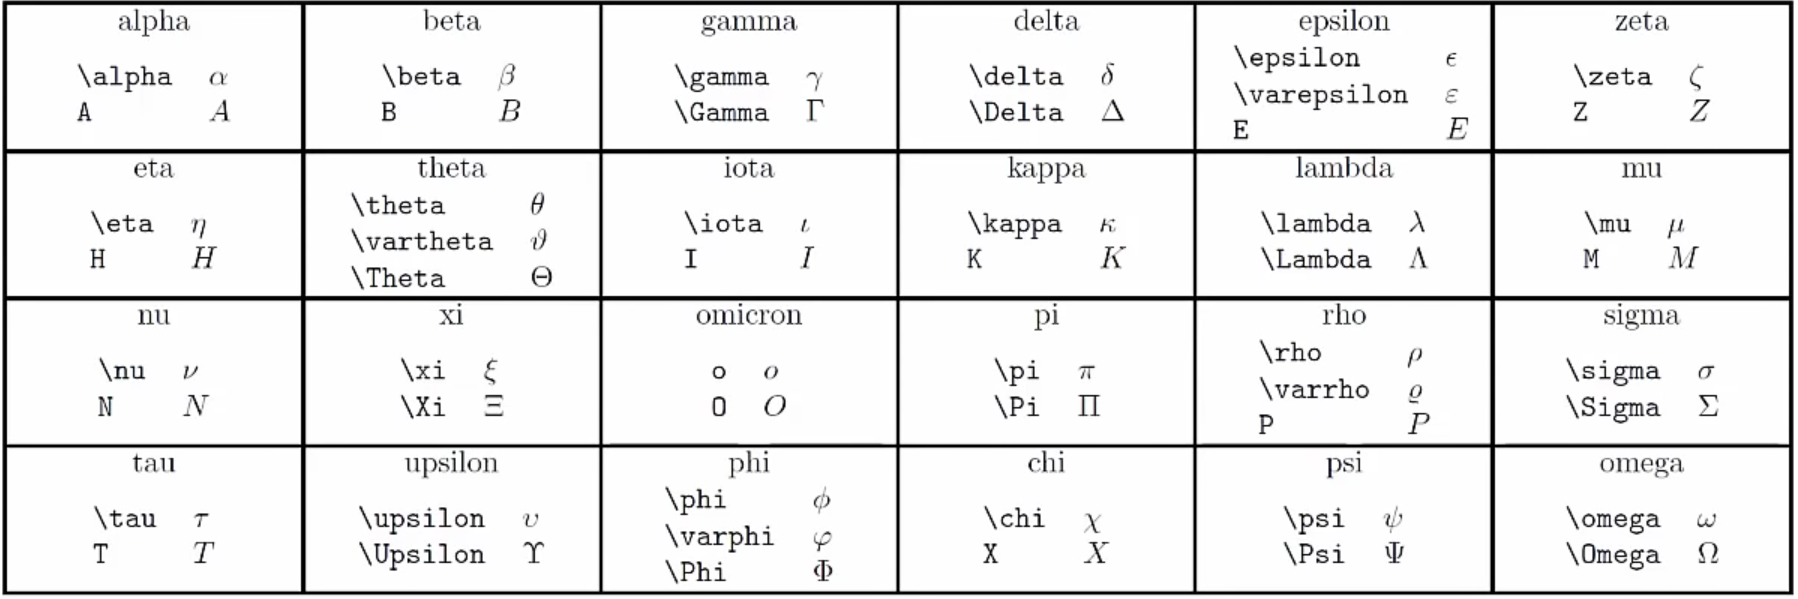
\includegraphics[scale=0.23]{greek_letters}
        \end{center}
        
            \href{https://detexify.kirelabs.org/classify.html}{\textbf{DeTeXify}} \href{https://detexify.kirelabs.org/classify.html}{(detexify.kirelabs.org/)} es una herramienta excelente para hallar simbolos cuyos nombres no recordemos.
        
    
    \subsection{Comandos útiles}
    
        Fuente, en general, utilizada para denotar cuerpos matemáticos. Se utiliza el comando \texttt{mathbb}.
            \[ 
                \begin{array}{c|c|c}
                	\text{Conjunto} & \text{Código} & \text{Output}\\
                	\hline
                	\text{Naturales} & \text{\texttt{\textbackslash mathbb \{N\}}} & \mathbb{N}\\
                	\text{Enteros} & \text{\texttt{\textbackslash mathbb \{Z\}}} & \mathbb{Z}\\
                	\text{Racionales} & \text{\texttt{\textbackslash mathbb \{Q\}}} & \mathbb{Q}\\
                	\text{Reales} & \text{\texttt{\textbackslash mathbb \{R\}}} & \mathbb{R}\\
                	\text{Complejos} & \text{\texttt{\textbackslash mathbb \{C\}}} & \mathbb{C}
                \end{array}
            \]
    
        Ejemplos para escribir distintos objetos.
        
        Polinomios:
            \begin{verbatim}
f(x) = a_n x^n + a_{n-1}  x^{n-1} + \cdots + a_1 x + a_0.
            \end{verbatim}
\[f(x) = a_n x^n + a_{n-1}  x^{n-1} + \cdots + a_1 x + a_0.
\]
        Exponenciales:
            \begin{verbatim}
f(x) = c_1 e^{r_1x} + c_2 e^{r_2 x}
            \end{verbatim}
\[f(x) = c_1 e^{r_1x} + c_2 e^{r_2 x}
\]
        Funcion de senos y cosenos sin funciones especiales:
            \begin{verbatim}
f(x) = cos x + i sin x
            \end{verbatim}
\[f(x) = f(x) = cos x + i sin x
\]
    Funcion de senos y cosenos con funciones especiales:
            \begin{verbatim}
f(x) = \cos x + i \sin x
            \end{verbatim}
\[f(x) = f(x) = \cos x + i \sin x
\]
        Nota: Para utilizar nombres de funciones personalizadas, se puede utilizar tanto los comandos \texttt{text} como \texttt{operatorname}.

        Suponga que desea escribir la siguiente fórmula matemática
            \[ \sum_{\substack{n = 0\\ n \text{ par}}} a_n x^n \]
        En una primera instancia, y con lo que hemos visto, uno tendería a escribir así
            \begin{verbatim}
\[ \sum_{n = 0\\ n \text{ par}} a_n x^n \]
            \end{verbatim}
        Esto arrojaría un error de compilación, por tanto no podriamos utilizarlo. Para esto, utilizamos el comando \texttt{substack}.
            \begin{verbatim}
\[ \sum_{\substack{n = 0\\ n \text{ par}}} a_n x^n \]
            \end{verbatim}
            
        Considere que desea escribir la siguiente fórmula
            \[ \iiint f(x,y,z) \, \mathrm{d}x \, \mathrm{d}y \, \mathrm{d}z \]
        En una primera instancia, y con lo que hemos visto, uno tendería a escribir así
            \begin{verbatim}
\[ \int\int\int f(x,y,z) dx dy dz \]
            \end{verbatim}
\[ \int\int\int f(x,y,z) dx dy dz \]
        Se tienen los comandos
        \[\begin{array}{cc}
            \text{\texttt{\textbackslash int}} & \displaystyle \int \\
            \text{\texttt{\textbackslash iint}} & \displaystyle\iint \\
            \text{\texttt{\textbackslash iiint}} & \displaystyle\iiint
        \end{array}\]
        
        Considere que desea escribir la siguiente fórmula
            \[ \iiint f(x,y,z) \, \mathrm{d}x \, \mathrm{d}y \, \mathrm{d}z \]
        Corrigiendo con lo que hemos visto
            \begin{verbatim}
\[ \iiint f(x,y,z) dx dy dz \]
            \end{verbatim}
\[ \iiint f(x,y,z) dx dy dz \]

    
        {\Large\[
        	\begin{array}{ccc}
                \text{} & \text{\texttt{f(x) dx}} & f(x) dx\\
                \text{\texttt{\textbackslash, }} & \text{\texttt{f(x) \textbackslash, dx}} & f(x) \, dx\\
                \text{\texttt{\textbackslash: }} & \text{\texttt{f(x) \textbackslash: dx}} & f(x) \: dx\\
                \text{\texttt{\textbackslash; }} & \text{\texttt{f(x) \textbackslash; dx}} & f(x) \; dx\\
                \text{\texttt{\textbackslash{}  }} & \text{\texttt{f(x) \textbackslash{}  dx}} & f(x) \ dx\\
                \text{\texttt{\textbackslash{}quad }} & \text{\texttt{f(x) \textbackslash quad dx}} & f(x) \quad dx
        	\end{array}
        \]}

        Considere que desea escribir la siguiente fórmula
            \[ \iiint f(x,y,z) \, \text{d}x \, \text{d}y \, \text{d}z \]
        Corrigiendo con lo que hemos visto
            \begin{verbatim}
\[ \iiint f(x,y,z) \, dx \, dy \, dz \]
            \end{verbatim}
\[ \iiint f(x,y,z) \, dx \, dy \, dz \]
        	¿Qué ocurre con la $d$? Usualmente con lo ya escrito bastaría. Pero para algunos, d es un operador y no una variable, por lo que se puede ser aún más detallista.
        {\footnotesize
            \begin{verbatim}
\[ \iiint f(x,y,z) \, \mathrm{d}x \, \mathrm{d}y \, \mathrm{d}z \]
            \end{verbatim}
        }
        
        	\[ \frac{\text{d}f}{\text{d}x} \]
\begin{verbatim}
\frac{\mathrm{d}f}{\mathrm{d}x}
\end{verbatim}
        	\underline{Notación Lagrangeana}
        	
        	\[   
        		\begin{array}{cc}      
        			\text{\texttt{f'(x)}} & f'(x)\\
        			\text{\texttt{f'}\texttt{'(x)}} & f''(x)\\
        			\text{\texttt{f'}\texttt{'}\texttt{'(x)}} & f'''(x)\\
        			\text{\texttt{f\^{}\{(n)\}(x)}} & f^{(n)}(x)\\
        		\end{array}
        	\]

        	\[ \frac{\partial f}{\partial x} \]
\begin{verbatim}
\frac{\partial f}{\partial x}
\end{verbatim}
        	\underline{Notación Newtoniana}
        	
        	\[   
        		\begin{array}{cc}      
        			\text{\texttt{\textbackslash{}dot\{x\}(t)}} & \dot{x}(t)\\
        			\text{\texttt{\textbackslash{}ddot\{x\}(t)}} & \ddot{x}(t)\\
        			\text{\texttt{\textbackslash{}dddot\{x\}(t)}} & \dddot{x}(t)\\
        			\text{\texttt{\textbackslash{}ddddot\{x\}(t)}} & \ddddot{x}(t)\\
        		\end{array}
        	\]
        
        El paquete \texttt{esvect} nos entrega utilidades para vectores.
        \[ \vv{r}(t) = \langle x(t), y(t), z(t) \rangle \]
        \begin{verbatim}
\vv{r}(t) = \langle x(t), y(t), z(t) \rangle
        \end{verbatim}
            
        \textbf{Ley de Inducción de Faraday}:
        \[ \vv{\nabla} \times \vv{E} = - \frac{\partial \vv{B}}{\partial t} \]
        \begin{verbatim}
\vv{\nabla} \times \vv{E} 
                = -\frac{\partial \vv{B}}{\partial t}
        \end{verbatim}
        \[ \oint \vv{E} \cdot \text{d}\vv{s} = \dfrac{\text{d} \Phi_B}{\text{d} t} \]
        \begin{verbatim}
\oint \vv{E} \cdot \mathrm{d}\vv{s} 
                = \dfrac{\mathrm{d} \Phi_B}{\mathrm{d} t} 
        \end{verbatim}            
        
    	
    		Los comandos del modo matemática son numerosos. Aún no se ha visto:
                \begin{enumerate}
                	\item Radicales.
                	\item Lógica y cuantificadores.
                	\item Relaciones de conjuntos.
                	\item Combinatoria.
                \end{enumerate}
            Como se ha dicho antes, se tendrán bastantes herramientas para poder encontrar la figura que se busca, como un buscador favorito, DeTeXify y listas grandes de comandos.\\[\baselineskip]
            
            \href{http://mirrors.rit.edu/CTAN/info/symbols/comprehensive/symbols-a4.pdf}{The Comprehensive \LaTeX{} Symbols List: http://mirrors.rit.edu/CTAN/info/symbols/comprehensive/symbols-a4.pdf}

        
\end{document}
